\section{Review of exam 1}%

\label{sec:Review of exam 1}
\subsection{Question 4}%
\label{sub:Question 4}
\[
\sum_{ n=1 } ^{ \infty } \frac{ \left( -1 \right) ^{ n+1 } }{ n+\sqrt{ n} }
.\] 
Using an absolute you can get rid of the absolute and use limit comparison to show 
\[
\lim_{ n \to \infty} \frac{ \frac{ 1 }{ n }  }{ \frac{ 1 }{ n+\sqrt{ n} }  }=\lim_{ n \to \infty} \frac{ n+\sqrt{ n} }{ n }=1
.\] 
Which means that both will either converge or diverge, but because $ \frac{ 1 }{ n }  $ is the harmonic we can see that both diverge and we can prove that it's conditional because AST shows that it's decreasing and limit is 0.
\subsection{Question 5}%
\label{sub:Question 5}
\[
\sum_{ n=2 } ^{ \infty } \frac{ 1 }{ n\left( n+2 \right)  } 
.\] 
Using partials we can deconstruct the series into 
\[
\sum_{ n=2 } ^{ \infty } \left( \frac{ 1 }{ 2n  } - \frac{ 1 }{ 2\left( n+2 \right)  }  \right) = \sum_{ n=2 } ^{ \infty } \frac{ 1 }{ 2 } \left( \frac{ 1 }{ n } -\frac{ 1 }{ n+2 }  \right) 
.\] 
Writing out terms you can see it becomes the telescoping
\[
\frac{ 1 }{ 2 } \left[ \left( \frac{ 1 }{ 2 } -\frac{ 1 }{ 4 }  \right) + \left( \frac{ 1 }{ 3 } -\frac{ 1 }{ 5 }  \right) + \ldots \right] 
.\] 
which cancels and leaves us with
\[
\frac{ 1 }{ 2 } \left[ \frac{ 1 }{ 2 } +\frac{ 1 }{ 3 }  \right] = \frac{ 5 }{ 12 } 
.\] 
\subsection{Question 7 friday}%
\label{sub:Question 7 friday}
\[
\ln^{  } \left( \sqrt{ 1-x^2} \right) 
.\] 
This can become $ \frac{ 1 }{ 2 } \ln^{  } \left( 1-x^2 \right)  $ and taking a $ \frac{ d }{ dx }  $ this becomes
\[
\frac{ 1 }{ 2 } \cdot \frac{ 1 }{ 1-x^2 } \cdot -2x= \frac{ -x }{ 1-x^2 } = -x\left( \frac{ 1 }{ 1-x^2 }  \right) =-\sum_{ n=0 } ^{ \infty } x^{ 2n+1 }
.\] 
Now taking the integral to reverse or derivative,
\[
\int_{  }^{  } -\sum_{ n=0 } ^{ \infty } x^{ 2n+1 }=-\sum_{ n=0 } ^{ \infty } \frac{ x^{ 2n+2 } }{ 2n+2 }
.\] 
Proving IOC can be done with ratio test as
\[
	\lim_{ n \to \infty} \left| \frac{ x^{ 2n+4 } }{ \cancel{ 2n+4 }} \cdot \frac{ 2n+2 }{ x^{ 2n+2 } } \right| = \left| x^2 \right| <1 \to -1<x<1 
.\] 

\section{Make a taylor without taylors thm }%
\label{sec:Make a taylor without taylors thm}
For $ e^{ x } $,
\[
1-x\le e^{ -x } \le 1
.\] 
\[
\int_{ 0 }^{ x } \left( 1-t \right) dt \le \int_{ 0 }^{ x } e^{ -t }dt \le \int_{ - }^{ x } 1dt
.\] 
\[
x-\frac{ x^2 }{ 2 } \le -e^{ -x }+1 \le x
.\] 
Integrate again,
\[
\int_{ 0 }^{ x } \left( t-\frac{ t^2 }{ 2 }  \right) dt\le \int_{ 0 }^{ x } \left( -e^{ -t }+1 \right) dt \le \int_{ 0 }^{ x } tdt
.\] 
\[
\frac{ x^2 }{ 2 } -\frac{ x^3 }{ 6 } \le e^{ x }+x \le 1 + \frac{ x^2 }{ 2 } 
.\] 
\[
1-x + \frac{ x^2 }{ 2 } -\frac{ x^3 }{ 6 } \le e^{ x } \le 1 -x +\frac{ x^2 }{ 2 } 
.\] 
Now we can use the squeeze theorem to show that $ e^{ x } $ is equal to the taylor series of $ e^{ x } $, or 
\[
e^{ x }= \sum_{ n=0 } ^{ \infty } \frac{ x^{ n } }{ n! }
.\] 
and
\[
e^{ -x }=\sum_{ n=0 } ^{ \infty } \frac{ \frac{ \left( -x \right) ^{ n } }{ \left( -1 \right) ^{ n }x^{ n } } }{ n! } 
.\] 
Which matches our created terms and shows that we made the MacLaurin series for $ e^{ x } $ without using the Taylor formula.
\section{Eulers formula (Tuesday)}%
\label{sec:Eulers formula}
Recall that the complex plain is a 2d plain that is comprised of a real and imaginary part, of $ a+\left( bi \right)  $ where $ i=\sqrt{ -1 }  $. This was used in pre-calc with quadratics like $ x^2+x+1=0 $ where our formula gets you to $ x = \frac{ -b\pm\sqrt{ b^2-4ac }  }{ 2a } = \frac{ -1\pm\sqrt{ -3 }  }{ 2 }\text{ or }\frac{ -1\pm\sqrt{ 3 } i }{ 2 } $. This can be graphed as points on complex plain and this helps with solving quadratics like this. \\

Going back to power series, if we write out the Maclaurin for $ e^{ x } $ and let our x be a complex number, $ a+bi $ we can write our sum as 
\[
e^{ a+bi } = e^{ a }+e^{ bi }= \sum_{ n=0 } ^{ \infty } \frac{ x^{ n } }{ n! }
.\] 
Prof went back on this to instead plot it as a vector with point $ \left( a, bi \right)  $ and angle of $ \theta $. Our magnitude or modulus would be $ \left| z \right|=\sqrt{ a^2+b^2 }  $ and our side lengths are $ \left| z \right|\sin^{  } \left( \theta \right)  $ and $ \left| z \right|\cos^{  } \left( \theta \right)  $. Now that we have this represenatation we can write it as
\[
\left| z \right|\cos^{  } \left( \theta \right) +i \left| z \right|\sin^{  } \left( \theta \right) 
.\] 
Which can be made into the below formula. 
\[
e^{ i \theta } \cos^{  } \left( \theta \right) + i \sin^{  } \left( \theta \right) 
.\] 
Proving this lets start with plugging in $ i\theta $ in for x in the series for $ e^{ x } $,
\[
	e^{ x }=e^{ i\theta }= \sum_{ n=0 } ^{ \infty } \frac{ \left( i\theta \right) ^{ n } }{ n! } = \frac{ i^{ 0 }\theta^{ 0 } }{ 0! }+ \frac{ i^{ 1 }\theta^{ 1 } }{ 1! }+ \frac{ i^{ 2 }\theta^{ 2 } }{ 2! }+ \frac{ i^{ 3 }\theta^{ 3 } }{ 3! } + \frac{ i^{ 4 }\theta^{ 4 } }{ 4! }+ \frac{ i^{ 5 }\theta^{ 5 } }{ 5! } + \frac{ i^{ 6 }\theta^{ 6 } }{ 6! } + \ldots
.\] 
Simplifying,
\[
1+i\theta - \frac{ 1 }{ 2! } \theta^2 - \frac{ i }{ 3! } \theta^3 + \frac{ 1 }{ 4! } \theta^4 + \frac{ i }{ 5! } \theta^5 - \frac{ 1 }{ 6! } \theta^6 - \ldots
.\] 
Now splitting it into our real and imaginary parts,
\[
1-\frac{ 1 }{ 2! } \theta^2+\frac{ \theta^{ 4 } }{ 4! }-\frac{ 1 }{ 6! } \theta^{ 6 }+ \ldots + i\left( \theta -\frac{ \theta^{ 3 } }{ 3! }+\frac{ \theta^{ 5 } }{ 5! }-\ldots \right) 
.\] 
Which can each be simplified to their respective maclaurins,
\[
\cos^{  } \left( \theta \right) \text{ and }i\sin^{  } \left( \theta \right) 
.\] 

\subsection{10.1 Intro to parametric equations}%
\label{sub:10.1 Intro to parametric equations}
Note that this will take around 2 weeks to cover so an exam can be expected around week 10-11. \\ \\ 

The idea is that we have a graph that is of the points $ \left( x,y \right)  $, but we cannot assign a function to it because the graph is not real, or there are more y points for each x and y is NOT a function of x. If we instead introduce another variable $ t $, we will have new sets of points that will be in terms of t and have points at $ \left( x\left( t \right) , y\left( t \right)  \right)  $ which will each be their own functions. For this case, we call our variable t a 'parameter' and this is what the root of parametric equations is, they are just the functions that define x and y over another parameter such as t or time. 

\ex{ Sketch the curve }
{ Given 
\begin{align*}
	x\left( t \right) &= 2t -4 \\
	y\left( t \right) &=3+t^2
.\end{align*}
For this we need to have a 3 column table that counts our t's and parametric equatiosn. Now we want to form a domain. Let's choose random t values to be $ -2,0,2,4 $. Now we can just plug these in to find our results for each parametric function. 
\begin{align*}
	x\left( t \right) &= -8,-4,0,4 \\
	y\left( t \right) &= 7,3,7,19 
.\end{align*}
Now that we have these points we can graph it to a 2d plain with coordinates $ \left( x\left( t \right) , y\left( t \right)  \right)  $. (i dont know how to use tikzpictures so i can't draw it here but its a quadratic going from left to right centered at $ \left( -4,3 \right)  $ ) This is really a three dimensional graph because we have 3 different variables but we won't draw the t dimension because it's linear and can just be represented like this for now. \\ \\
} 
\newpage
Now that we did it by hand, we can also do it with a calculator. Start with going to mode and selecting 'PAR' instead of 'FUNC'. This will put you into parametric mode and now the $ y= $ will have another dimension inside of it. Now we can input our sets of equations in for what the calculator wants. Now that the values are in the functions, we can make our window mins to be our domain of t, which we can recall to be $ \left[ -2,4 \right]  $ and we can input our step size to be 2 because of our previous points. Again looking at the graph I DIDNT DRAW, we can see our $ x_{ min } $ can be around -10 and $ x_{ max } $ to be around 6. Doing the same thing for y we can write it as $ 0 $ and 20. \\ \\

Now graphing it we can see that it looks around the same as how I TOTALLY DREW IT AS. Now if we decrease the step size we get a smoother and smoother curve, with the absolute curve being $ \lim_{ t \to \infty} \left( x\left( t \right) , y\left( t \right)  \right)  $. Choosing a VERY low value of t will make the calculator work for a while so 0.25 is suggested to get a decent looking curve. 
\subsection{Removing the parameter}%
\label{sub:Removing the parameter}
With our previous example again, 
\begin{align*}
	x\left( t \right) &= 2t -4 \\
	y\left( t \right) &=3+t^2
.\end{align*}
We can solve for t and substitute it into the other equation to get a function of x and y.

\[
	x+4=2t \to t=\frac{ x+4 }{ 2 } \text{ and } y=3+\left( \frac{ x+4 }{ 2 } \right) ^2
.\] 
We can now instead graph this and we get the same function. This is just algebra again\ldots but this doesn't always work so that's why this section of calc exists I guess.
\subsection{Wednesday, cont. of intro to parametric equations}%
\label{sub:Wednesday, cont. of intro to parametric equations}
\dfn{ Ways to make a line with parametrics}{ 
\paragraph{a) A line through (a,b) with slope m.}
\[
x\left( t \right) =a+rt , y\left( t \right) =b+st
.\] 
Where $ m=\frac{ s }{ r }  $. \\ \\

\paragraph{b) Parametrize across two points}
 \[
p=\left( a,b \right) ; Q = \left( c,d \right) 
.\] 
For $ t\epsilon\left[ 0,1 \right]  $,
\[
x\left( t \right) =a+t\left( c-a \right) , y\left( t \right) =b+t\left( d-b \right)
.\] \\ \\
\paragraph{c) In general, $ p\to Q $ and $ t_1 \to t_2 $ for $ \left[ t_1,t_2 \right]  $}
\[
x\left( t \right) = a + \frac{ t-t_1 }{ t_2-t_1 }\left( c-a \right) 
.\] 
\[
y\left( t \right) = b + \frac{ t-t_1 }{ t_2-t_1 }\left( d - b \right) 
.\] 

}
\ex{ (1,3) = point $ m=\frac{ 2 }{ 5 }  $ }{ 
With our formula you can write our parametric equations as
\[
x\left( t \right) =1+5t
.\] 
\[
y\left( t \right) =3+2t
.\] 
Solving for the $ y=mx+b $ version,
\begin{align*}
	y-y_1 &= m\left( x-x_1 \right) \\
y-3 &= \frac{ 2 }{ 5 } \left( x-1 \right)  \\
y&= \frac{ 2 }{ 5 } x +\frac{ 13 }{ 5 } 
.\end{align*}
Using the normal method we can do it as 
\[
y\left( t \right) =3+2\left( \frac{ x-1 }{ 5 } \right) = \frac{ 2 }{ 5 } x + \frac{ 13 }{ 5 } 
.\] 
} 
\dfn { Basic way to turn $ y=f\left( x \right)  $ into a parametric }{ 
	\begin{align*}
		y=f\left( x \right) &\to x\left( t \right) =t\\
	&\to y\left( t \right) =f\left( t \right)
	.\end{align*}
} 
\subsection{Circles}%
\label{sub:Circles}
If we have a circle of radius 1 and define our $ \theta $ as t or time, we know that our coordinate is literally $ \left( \cos^{  } \left( t \right) ,\sin^{  } \left( t \right)  \right)  $. Moving the circle to be centered somewhere that isn't 0 would be done by having the coordinates become
\[
\left( h+r\cos^{  } \left( t \right) ,k+r\sin^{  } \left( t \right)  \right)
.\] 
Where h and k are the center points and r will be the radius. This can be used to find any normal circle. This however, will trace clockwise and is fine for most cases, but if we wanted to do it as going the opposite direction while still going in forward time, we instead use 
\[
	\left( r\sin^{  } \left( t \right) , r\cos^{  } \left( t \right)  \right) \text{ or }\left( r\cos^{  } \left( -t \right) ,r\sin^{  } \left( -t \right)  \right) = \left( r\cos^{  } \left( t \right) -r\sin^{  } \left( t \right)  \right) 
.\] 
So to get around the circle one time we would need $ t\epsilon\left[ 2\pi \right]  $. If we instead wanted it to trace in half the time or $ t\epsilon\left[ 0,\pi  \right]  $, we can call our coordinates
\[
	\left( r\cos^{  } \left( 2t \right) ,r\sin^{  } \left( 2t \right)  \right) 
.\] 
\subsection{Ellipse}%
\label{sub:Ellipse}
With our major (a) and minor (b) axis, if we let our coordinates be $ \left( a\cos^{  } \left( t \right) , b\sin^{  } \left( t \right)  \right)  $ we can draw ellipses. It can also be shifted by just adding an h and k for the centers. 
\newpage
\section{Thursday, 10.1 parametric eqs. cont}%
\label{sec:Thursday, 10.1 parametric eqs. cont}
\ex{ }{ 
	\paragraph{Ex.} A turtle walks constant speed counter-clockwise on circular path, radius 4ft, centered at $ \left( 0,0 \right)  $. Turtle starts at $ \left( 4,0 \right)  $ and completes one lap in 30 minutes. Let t be minutes $ t\ge 0 $.  \\ \\
	Start with the basic coords of a circle, 
	\[
		\left( x\left( t \right) ,y\left( t \right)  \right) =\left( 4\cos^{  } \left( bt \right) ,4\sin^{  } \left( bt \right)  \right) 
	.\] 
	Solve for b, $ \frac{ 2 \pi  }{ b } \to b = \frac{ \pi }{ 15 }   $, so $ t\epsilon\left[ 0,30 \right]  $. 
} 

\subsection{Physics: Projectile motion in two dimensions}%
\label{sub:Physics: Projectile motion in two dimensions}
If we know the vector (magnitude and angle) of an object and we neglect air resistance, and call each component of the vector ($ v_0 $) as vectors $ \left( tv_0\cos^{  } \left( \theta \right) ,tv_0\sin^{  } \left( \theta \right)  \right)  $, because we also want gravity we call our y vector $ tv_0\sin^{  } \left( \theta \right) -\frac{ 1 }{ 2 } 9.81t^2 $. 

\ex{ A baseball is hit with a bat }{ 
\begin{gather*}
v_0=150 \frac{ ft }{ s } , \theta= 35^{\circ} , h = 3ft
\end{gather*}
So now our balls position as a function of time is written as 
\[
	\left( 150\cos^{  } \left( 35 \right) t, 150\sin^{  } \left( 35 \right) t-\frac{ 1 }{ 2 } \left( 32 \right) t^2 + 3\right) 
.\] 
The rest of the question is basic physics, part a included plugging in values of t to find some points of the ball and part was taking the $ \frac{ d }{ dx }  $ of the y component to find the maximum when the velocity is at 0. This goes to $ 150\sin^{  } \left( 35 \right) -32t  $ and $ t=\frac{ 150\sin^{  } \left( 35 \right)  }{ 32 } $. This can also be plugging into calculator to find it. \\ \\
For part c we want to set the quadratic to 0 for when $ y=0 $ and plug that t back into the position of x to find the distance it went. 

} 
\section{Friday 2/28}%
\label{sec:Friday 2/28}
\subsection{Calculus with parametric cords.}%
\label{sub:Calculus with parametric cords.}


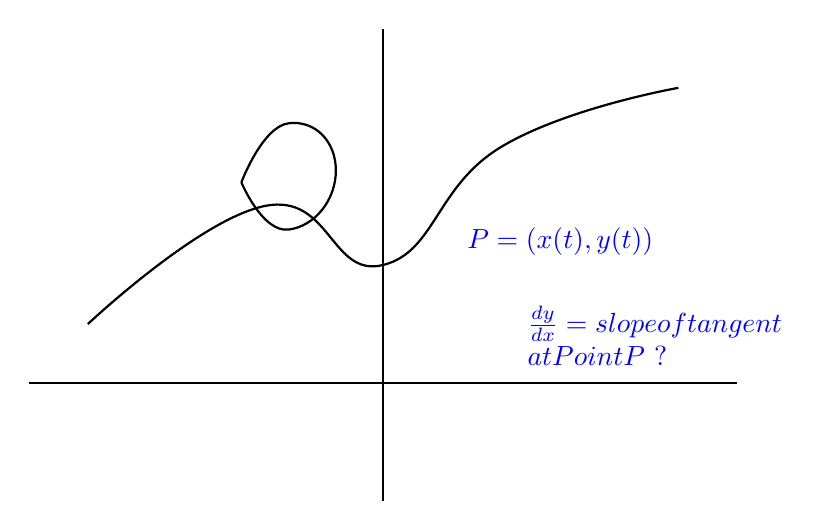
\begin{tikzpicture}[scale=1.5]
    % Draw coordinate axes
    \draw[thick] (-3,0) -- (3,0);
    \draw[thick] (0,-1) -- (0,3);
    
    % Draw the curve with a loop
    \draw[white, thick] plot[smooth, tension=0.8] coordinates {(-2.5,0.5) (-1,1.5) (0,1) (1,2) (2.5,2.5)};
    
    % Redraw the curve in black
    \draw[thick] plot[smooth, tension=0.8] coordinates {(-2.5,0.5) (-1,1.5) (0,1) (1,2) (2.5,2.5)};
    
    % Add the loop to the curve
    \draw[thick] plot[smooth, tension=1] coordinates {(-1.2,1.7) (-0.8,2.2) (-0.4,1.8) (-0.8,1.3) (-1.2,1.7)};
    
    % Add the tangent arrow
    
    % Add blue annotations for the point and formula
    \node[blue] at (1.5,1.2) {$P = (x(t), y(t))$};
    
    % Add blue derivative annotation
    \node[blue, align=left] at (2.3,0.4) {$\frac{dy}{dx} = \text{slope of tangent}$\\$\text{at Point }P$ ?};
    
\end{tikzpicture} \\ \\
Picture was something like the above and was there to show that the tangent of the circle will be $ \frac{ dy }{ dx }  $ at any point p. 
\dfn { First $ \frac{ d }{ dx } proof parametrics $ }{ 
Starting with a function, we can take it's $ \frac{ d }{ dx }  $ with respect to time as,
\[
\frac{ dy }{ dt } 
.\] 
Which can then be expanded to
\[
=\frac{ dy }{ dx } \cdot \frac{ dx }{ dt } 
.\] 
and made into
\[
\to \frac{ dy }{ dx } = \frac{ \frac{ dy }{ dt }  }{ \frac{ dx }{ dt }  }= \frac{ y'\left( t \right)  }{ x'\left( t \right)  }
.\] 
if $ x'\left( t \right) \neq 0 $. \\ \\ 

\paragraph{For the second $ \frac{ d }{ dx }  $}
By quotient rule we can take the second $ \frac{ d }{ dx }  $ as,
\[
D\left( \frac{ dy }{ dx }  \right) = \frac{ d^2y }{ dx^2 } = \frac{ d }{ dx } \left( \frac{ dy }{ dx }  \right) = \frac{ \frac{ d }{ dt } \left( \frac{ dy }{ dx } \right)  }{ \frac{ dx }{ dt }  }= \frac{ \frac{ d }{ dt } \left( \frac{ y'\left( t \right)  }{ x'\left( t \right)  } \right)  }{ x'\left( t \right)  } = \frac{ x'\left( t \right) \cdot y''\left( t \right) - y'\left( t \right) \cdot x''\left( t \right)  }{ \left( x'\left( t \right)  \right) ^3 }
.\] 
} 
The above has use cases for finding derivatives of our parametrics and lets say we were to use them in a circle with $ t= \frac{ 5 \pi  }{ 4 } $. \\ \\

Using the above formula we take the derivative of sin and cos and plug them in to find,
 \[
 \frac{ dy }{ dx } =\frac{ y'\left( t \right)  }{ x'\left( t \right)  }= \frac{ -\cos^{  } \left( t \right)  }{ -\sin^{  } \left( t \right)} = \frac{ \frac{ \sqrt{ 2 }  }{ 2 } }{ \frac{ \sqrt{ 2 }  }{ 2 } }= 1
.\] 
will be our tangent. 
